\section{Tinjauan Pustaka}
\subsection{Arsitektur Famili YOLO}
  \subsubsection{\emph{Layer Head} YOLO dan \emph{Anchor Box}}
    \begin{figure}[ht]
        \centering
        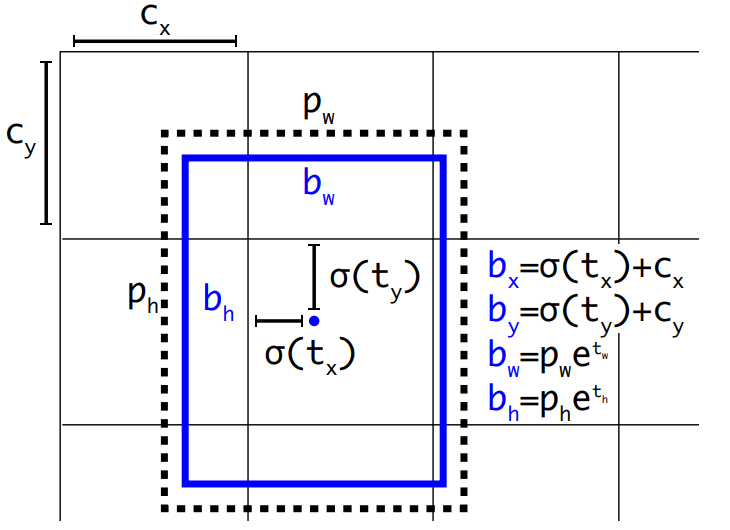
\includegraphics[scale=0.4]{pictures/anchorbox.png}
        \caption{Prediksi \emph{Anchor Box} dan \emph{offset} dari koordinat latis}
        \label{fig:anchorbox}
    \end{figure}
    Semenjak YOLO9000, arsitektur famili YOLO yang dipublikasikan setelahnya terus menggunakan \emph{anchor box} untuk melakukan deteksi \parencites{yolov2}{yolov3}{yolov4}{scaledyolov4}{yolov5}{yolor}{yolov7}.
    \emph{Anchor boxes} merupakan beberapa \emph{Bounding Box} yang telah terdefinisikan. 
    Arsitektur YOLO akan memprediksi probabilitas \emph{anchor box} berada pada suatu koordinat latis beserta dengan \emph{offset anchor box} tersebut untuk menepatkan \emph{anchor box} pada objek yang dideteksi.
    Penggunaan \emph{anchor box} ini dapat meningkatkan akurasi deteksi karena \emph{neural network} hanya perlu mencari titik tengah objek dan \emph{error} dimensi \emph{boudning box} dengan menggunakan \emph{offset} \parencite{yolov3}.
    Hal ini lebih sederhana daripada mencari titik-titik \emph{bounding box} secara independen sehingga lebih mudah untuk dipelajari oleh \emph{neural network}.

    Prediksi \emph{bounding boxes} terjadi di bagian \emph{head} dari arsitektur YOLO.
    Bagian \emph{head} dari YOLO akan mengambil beberapa hasil \emph{upsampling} yang terjadi pada \emph{neck} YOLO, dan kemudian melakukan prediksi \emph{anchor boxes} dari hasil tersebut.
    Hasil prediksi \emph{Head} YOLO pada suatu tingkatan \emph{upsampling} berupa tensor dengan ukuran $N\times N \times [A\times(4+1+C)]$ dengan $N$ sebagai dimensi hasil \emph{upsampling}-nya, $A$ sebagai jumlah \emph{anchor boxes} untuk \emph{scaling} tersebut, dan $C$ sebagai jumlah kelas prediksi.
    Angka 4 merepresentasikan 4 \emph{offset} $b_x, b_y, b_w, b_h$ seperti pada Gambar \ref{fig:anchorbox} dan angka 1 merepresentasikan \emph{objectness score} dari prediksi \emph{bounding box}.

  \subsubsection{\emph{Neck} YOLO}

    \begin{figure}[ht]
        \centering
        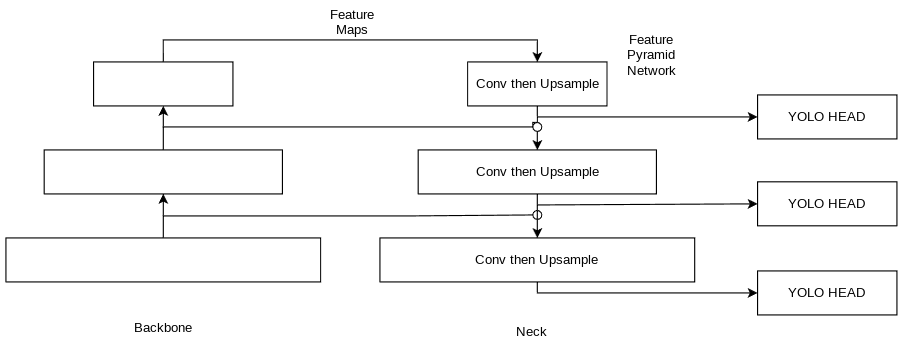
\includegraphics[scale=0.6]{pictures/yolo-architecture-rough.png}
        \caption{\emph{Feature Pyramid Network} pada \emph{Neck} YOLO}
        \label{fig:yolofpn}
    \end{figure}

    \emph{Neck} dari YOLO merupakan \emph{layer-layer} dimana \emph{head} YOLO mengambil fitur untuk dilakukan deteksi \emph{bounding box}.
    Pada YOLOv3 \textcite{yolov3}, arsitektur \emph{neck} dibuat menyerupai \emph{Feature Pyramid Network} (FPN) seperti pada Gambar \ref{fig:yolofpn}. 
    Pada versi-versi YOLO selanjutnya, bentuk \emph{neck} ini tidak banyak berubah.

    Penaikkan tingkatan \emph{pyramid} dari FPN merupakan \emph{upsampling} dari \emph{feature map} yang dihasilkan \emph{backbone}.
    Output tiap tingkatan pada FPN di \emph{neck} inilah yang diinputkan pada \emph{head} YOLO. 
    Melakukan prediksi pada tingkatan \emph{upsampling} yang berbeda-beda dapat membuat \emph{neural network} mendapatkan lebih banyak informasi semantik dan informasi yang lebih detail sehingga dapat lebih akurat dalam mendeteksi objek besar maupun kecil.

  \subsubsection{\emph{Backbone} YOLO}
    \emph{Backbone} dari YOLO merupakan bagian yang mengekstrak fitur dari citra yang diinputkan.
    Hasil ekstraksi fitur ini akan diinputkan pada \emph{neck} yang kemudian akan di\emph{upsampling} olehnya.
    Model-model YOLO dapat menggunakan \emph{feature extractor} dari model-model klasifikasi citra sebagai \emph{backbone}-nya.
    Sebagai contoh, salah satu varian YOLO, YOLO-Z menggunakan ResNet-50 sebagai \emph{backbone}-nya sedangkan arsitektur YOLO dasarnya, YOLOv5 menggunakan CSP-Darknet \parencite{yoloz}.




\subsection{YOLOv7}
  \lipsum[1]
\subsection{Rekalkulasi Anchor}
  \lipsum[1]
\subsection{Augmentasi \emph{Mosaic}}
  \lipsum[1]

\subsection{Penelitian Terkait}
  \subsubsection{YOLO-Z}
    \lipsum[2]
  \subsubsection{exYOLO}
    \lipsum[2]
  \subsubsection{Penelitian si orang slavic yg menang lomba}
    \lipsum[2]